%---------------
%╔═╗╔═╗╔╦╗╦  ╦╔═╗
%╚═╗║╣    ║  ║  ║╠═╝
%╚═╝╚═╝  ╩  ╚═╝╩  
%---------------

% language setup
\newcommand{\docLanguage}{ngerman}
%\newcommand{\docLanguage}{english}

% DOCUMENT SETUP
\documentclass[12pt, oneside, a4paper, \docLanguage]{report}
\usepackage[left=3cm, 
			right=2.5cm, 
			top=2.5cm, 
			bottom=2.5cm, 
			includehead, 
			includefoot]{geometry}

% line spacing
\usepackage{setspace}
\setstretch{1,25} % 15/12 --> 1.25

% encoding setup
% T1 font encoding for languages that use a latin alphabet
\usepackage[T1]{fontenc} 

% enhanced input encoding handling - utf8 for äÄüÜöÖß...
\usepackage[utf8]{inputenc}

%de­fines Adobe Times Ro­man as de­fault text font
\usepackage{mathptmx}
\usepackage{times} % needed for acronym package

%PDF linking package
\usepackage[hidelinks]{hyperref}


% Language Setup
\usepackage[\docLanguage]{babel}
% after babel - set chapter string
\AtBeginDocument{\renewcommand{\chaptername}{}}

% language specific bibliography style
\usepackage[numbers, square]{natbib}
%\setcitestyle{square,aysep={},yysep={;}}
\usepackage[fixlanguage]{babelbib}
\selectbiblanguage{\docLanguage}
% bliographystyle setup
% babel specific: babplain, babplai3, babalpha, babunsrt, bababbrv, bababbr3
\bibliographystyle{babunsrt}


% enumeration
\usepackage{enumitem}
% tabular extension tabularx
\usepackage{tabularx}

% math packages
\usepackage{amsmath}
\usepackage{nicefrac}
\usepackage{amsthm}
\usepackage{amsbsy}
\usepackage{amssymb}
\usepackage{amsfonts}
%\usepackage{MnSymbol}


%special characters
\usepackage{amssymb}
\usepackage{upgreek,textgreek}

% acronym package
\usepackage[printonlyused, footnote]{acronym}

% breakable text in \seqsplit{}
\usepackage{seqsplit}

% \textmu
\usepackage{textcomp}

% package provides a way to compile sections of a document using the same preamble as the main document
\usepackage{subfiles}

% driver-independent color extension - used by listings,tabularx
\usepackage[usenames,dvipsnames,table,xcdraw]{xcolor}

% -- SYNTAX HIGHLIGHTING --
\usepackage{listings}
%% bash command line Syntax Highlighting
\lstdefinestyle{BASH_CMD}{ 
  columns=fullflexible,            % copy pasteable listings
  language=bash,
  basicstyle=\small\sffamily,
  basicstyle   = \small \ttfamily,
  keywordstyle = [1]\small \ttfamily,
  keywordstyle = [2]\small \ttfamily,
  commentstyle = \small \ttfamily,
  numbers=none,
  captionpos=b, 
  breaklines=true,
  numberstyle=\tiny,
  numbersep=3pt,
  frame=tlrb,
  columns=fullflexible,
  backgroundcolor=\color{white!20},
  linewidth=\linewidth,
  literate=                        % replace in code
     {Ö}{{\"O}}1 
     {Ä}{{\"A}}1 
     {Ü}{{\"U}}1 
     {ß}{{\ss}}2 
     {ü}{{\"u}}1 
     {ä}{{\"a}}1 
     {ö}{{\"o}}1 
     {â}{{\^{a}}}1 
     {Â}{{\^{A}}}1 
     {ç}{{\c{c}}}1 
     {Ç}{{\c{C}}}1 
     {ğ}{{\u{g}}}1 
     {Ğ}{{\u{G}}}1 
     {ı}{{\i}}1 
     {İ}{{\.{I}}}1 
     {ş}{{\c{s}}}1 
     {Ş}{{\c{S}}}1 
}
 % adds style BASH_CMD
%% Matlab Syntax Highlighting
\colorlet{keyword}{blue!100!black!80}
\colorlet{STD}{Lavender}
\colorlet{comment}{green!90!black!90}
\definecolor{mygreen}{rgb}{0,0.6,0}
\definecolor{mygray}{rgb}{0.5,0.5,0.5}
\definecolor{mymauve}{rgb}{0.58,0,0.82}


\lstdefinestyle{BASH_SCRIPT}{ 
  language     = bash,
  basicstyle   = \footnotesize \ttfamily,
  keywordstyle = [1]\color{keyword}\bfseries,
  keywordstyle = [2]\color{STD}\bfseries,
  commentstyle = \color{mygreen}\itshape,
  backgroundcolor=\color{white},   % choose the background color; you must add \usepackage{color} 
  columns=fullflexible,            % copy pasteable listings
                                   % or \usepackage{xcolor}
  basicstyle=\footnotesize,        % the size of the fonts that are used for the code
  breakatwhitespace=false,         % sets if automatic breaks should only happen at whitespace
  breaklines=true,                 % sets automatic line breaking
  captionpos=b,                    % sets the caption-position to bottom
  extendedchars=true,              % lets you use non-ASCII characters; for 8-bits encodings only,
                                   % does not work with UTF-8
  frame=single,                    % adds a frame around the code
  keepspaces=true,                 % keeps spaces in text, useful for keeping indentation of code
                                   % (possibly needs columns=flexible)
  numbers=left,                    % where to put the line-numbers; possible values are 
                                   % (none, left, right)
  numbersep=5pt,                   % how far the line-numbers are from the code
  numberstyle=\tiny\color{mygray}, % the style that is used for the line-numbers
  rulecolor=\color{black},         % if not set, the frame-color may be changed on line-breaks
                                   % within not-black text (e.g. comments (green here))
  showspaces=false,                % show spaces everywhere adding particular underscores; it
  	                               % overrides 'showstringspaces'
  showstringspaces=false,          % underline spaces within strings only
  showtabs=false,                  % show tabs within strings adding particular underscores
  stepnumber=1,                    % the step between two line-numbers. If it's 1, each line 
                                   % will be numbered
  stringstyle=\color{mymauve},     % string literal style
  tabsize=2,                       % sets default tabsize to 2 spaces
  title=\lstname,                  % set title name
  literate=                        % replace in code
     {Ö}{{\"O}}1 
     {Ä}{{\"A}}1 
     {Ü}{{\"U}}1 
     {ß}{{\ss}}2 
     {ü}{{\"u}}1 
     {ä}{{\"a}}1 
     {ö}{{\"o}}1 
     {â}{{\^{a}}}1 
     {Â}{{\^{A}}}1 
     {ç}{{\c{c}}}1 
     {Ç}{{\c{C}}}1 
     {ğ}{{\u{g}}}1 
     {Ğ}{{\u{G}}}1 
     {ı}{{\i}}1 
     {İ}{{\.{I}}}1 
     {ş}{{\c{s}}}1 
     {Ş}{{\c{S}}}1 
} % adds style BASH_SCRIPT
% Matlab Syntax Highlighting
\colorlet{keyword}{blue!100!black!80}
\colorlet{STD}{red}
\colorlet{comment}{green!90!black!90}
\definecolor{mygreen}{rgb}{0,0.6,0}
\definecolor{mygray}{rgb}{0.5,0.5,0.5}
\definecolor{mymauve}{rgb}{0.58,0,0.82}


\lstdefinestyle{LATEX}{ 
  language     = [LaTeX]{TeX},
  basicstyle   = \footnotesize \ttfamily,
  keywordstyle = [1]\color{keyword}\bfseries,
  keywordstyle = [2]\color{comment}\bfseries,
  commentstyle = \color{mygray}\itshape,
  %backgroundcolor=\color{white},   % choose the background color; you must add \usepackage{color} 
                                   % or \usepackage{xcolor}
  basicstyle=\footnotesize,        		   % the size of the fonts that are used for the code
  breakatwhitespace=false,         % sets if automatic breaks should only happen at whitespace
  columns=fullflexible,            % copy pasteable listings
  breaklines=true,                 % sets automatic line breaking
  captionpos=c,                    % sets the caption-position to bottom
  extendedchars=true,              % lets you use non-ASCII characters; for 8-bits encodings only,
                                   % does not work with UTF-8
  frame=single,                    % adds a frame around the code
  keepspaces=true,                 % keeps spaces in text, useful for keeping indentation of code
                                   % (possibly needs columns=flexible)
  numbers=left,                    % where to put the line-numbers; possible values are 
                                   % (none, left, right)
  numbersep=4pt,                   % how far the line-numbers are from the code
  numberstyle=\tiny\color{mygray}, % the style that is used for the line-numbers
  rulecolor=\color{black},         % if not set, the frame-color may be changed on line-breaks
                                   % within not-black text (e.g. comments (green here))
  showspaces=false,                % show spaces everywhere adding particular underscores; it
  	                               % overrides 'showstringspaces'
  showstringspaces=false,          % underline spaces within strings only
  showtabs=false,                  % show tabs within strings adding particular underscores
  stepnumber=1,                    % the step between two line-numbers. If it's 1, each line 
                                   % will be numbered
  stringstyle=\color{mymauve},     % string literal style
  tabsize=2,                       % sets default tabsize to 2 spaces
  title=\lstname,                  % set title name
  literate=                        % replace in code
     {Ö}{{\"O}}1 
     {Ä}{{\"A}}1 
     {Ü}{{\"U}}1 
     {ß}{{\ss}}2 
     {ü}{{\"u}}1 
     {ä}{{\"a}}1 
     {ö}{{\"o}}1 
     {â}{{\^{a}}}1 
     {Â}{{\^{A}}}1 
     {ç}{{\c{c}}}1 
     {Ç}{{\c{C}}}1 
     {ğ}{{\u{g}}}1 
     {Ğ}{{\u{G}}}1 
     {ı}{{\i}}1 
     {İ}{{\.{I}}}1 
     {ş}{{\c{s}}}1 
     {Ş}{{\c{S}}}1 
} % adds style LATEX
%% Matlab Syntax Highlighting
\colorlet{keyword}{blue!100!black!80}
\colorlet{STD}{Lavender}
\colorlet{comment}{green!90!black!90}
\definecolor{mygreen}{rgb}{0,0.6,0}
\definecolor{mygray}{rgb}{0.5,0.5,0.5}
\definecolor{mymauve}{rgb}{0.58,0,0.82}


\lstdefinestyle{MATLAB}{ 
  language     = Matlab,
  basicstyle   = \footnotesize \ttfamily,
  keywordstyle = [1]\color{keyword}\bfseries,
  keywordstyle = [2]\color{STD}\bfseries,
  commentstyle = \color{mygreen}\itshape,
  backgroundcolor=\color{white},   % choose the background color; you must add \usepackage{color} 
                                   % or \usepackage{xcolor}
  basicstyle=\footnotesize,        % the size of the fonts that are used for the code
  breakatwhitespace=false,         % sets if automatic breaks should only happen at whitespace
  columns=fullflexible,            % copy pasteable listings
  breaklines=false,                % sets automatic line breaking
  captionpos=c,                    % sets the caption-position to bottom
  extendedchars=true,              % lets you use non-ASCII characters; for 8-bits encodings only,
                                   % does not work with UTF-8
  frame=single,                    % adds a frame around the code
  keepspaces=true,                 % keeps spaces in text, useful for keeping indentation of code
                                   % (possibly needs columns=flexible)
  numbers=left,                    % where to put the line-numbers; possible values are 
                                   % (none, left, right)
  numbersep=5pt,                   % how far the line-numbers are from the code
  numberstyle=\tiny\color{mygray}, % the style that is used for the line-numbers
  rulecolor=\color{black},         % if not set, the frame-color may be changed on line-breaks
                                   % within not-black text (e.g. comments (green here))
  showspaces=false,                % show spaces everywhere adding particular underscores; it
  	                               % overrides 'showstringspaces'
  showstringspaces=false,          % underline spaces within strings only
  showtabs=false,                  % show tabs within strings adding particular underscores
  stepnumber=1,                    % the step between two line-numbers. If it's 1, each line 
                                   % will be numbered
  stringstyle=\color{mymauve},     % string literal style
  tabsize=2,                       % sets default tabsize to 2 spaces
  title=\lstname,                  % set title name
  literate=                        % replace in code
     {Ö}{{\"O}}1 
     {Ä}{{\"A}}1 
     {Ü}{{\"U}}1 
     {ß}{{\ss}}2 
     {ü}{{\"u}}1 
     {ä}{{\"a}}1 
     {ö}{{\"o}}1 
     {â}{{\^{a}}}1 
     {Â}{{\^{A}}}1 
     {ç}{{\c{c}}}1 
     {Ç}{{\c{C}}}1 
     {ğ}{{\u{g}}}1 
     {Ğ}{{\u{G}}}1 
     {ı}{{\i}}1 
     {İ}{{\.{I}}}1 
     {ş}{{\c{s}}}1 
     {Ş}{{\c{S}}}1 
} % adds style MATLAB
% Matlab Syntax Highlighting
\colorlet{keyword}{blue!100!black!80}
\colorlet{STD}{Lavender}
\colorlet{comment}{green!90!black!90}
\definecolor{mygreen}{rgb}{0,0.6,0}
\definecolor{mygray}{rgb}{0.5,0.5,0.5}
\definecolor{mymauve}{rgb}{0.58,0,0.82}


\lstdefinestyle{PYTHON}{ 
  language     = Python,
  basicstyle   = \footnotesize \ttfamily,
  keywordstyle = [1]\color{keyword}\bfseries,
  keywordstyle = [2]\color{STD}\bfseries,
  commentstyle = \color{mygreen}\itshape,
  backgroundcolor=\color{white},   % choose the background color; you must add \usepackage{color} 
                                   % or \usepackage{xcolor}
  basicstyle=\footnotesize,        % the size of the fonts that are used for the code
  columns=fullflexible,            % copy pasteable listings
  breakatwhitespace=false,         % sets if automatic breaks should only happen at whitespace
  breaklines=false,                % sets automatic line breaking
  captionpos=c,                    % sets the caption-position to bottom
  extendedchars=true,              % lets you use non-ASCII characters; for 8-bits encodings only,
                                   % does not work with UTF-8
  frame=single,                    % adds a frame around the code
  keepspaces=true,                 % keeps spaces in text, useful for keeping indentation of code
                                   % (possibly needs columns=flexible)
  numbers=left,                    % where to put the line-numbers; possible values are 
                                   % (none, left, right)
  numbersep=5pt,                   % how far the line-numbers are from the code
  numberstyle=\tiny\color{mygray}, % the style that is used for the line-numbers
  rulecolor=\color{black},         % if not set, the frame-color may be changed on line-breaks
                                   % within not-black text (e.g. comments (green here))
  showspaces=false,                % show spaces everywhere adding particular underscores; it
  	                               % overrides 'showstringspaces'
  showstringspaces=false,          % underline spaces within strings only
  showtabs=false,                  % show tabs within strings adding particular underscores
  stepnumber=1,                    % the step between two line-numbers. If it's 1, each line 
                                   % will be numbered
  stringstyle=\color{mymauve},     % string literal style
  tabsize=2,                       % sets default tabsize to 2 spaces
  title=\lstname,                  % set title name
  literate=                        % replace in code
     {Ö}{{\"O}}1 
     {Ä}{{\"A}}1 
     {Ü}{{\"U}}1 
     {ß}{{\ss}}2 
     {ü}{{\"u}}1 
     {ä}{{\"a}}1 
     {ö}{{\"o}}1 
     {â}{{\^{a}}}1 
     {Â}{{\^{A}}}1 
     {ç}{{\c{c}}}1 
     {Ç}{{\c{C}}}1 
     {ğ}{{\u{g}}}1 
     {Ğ}{{\u{G}}}1 
     {ı}{{\i}}1 
     {İ}{{\.{I}}}1 
     {ş}{{\c{s}}}1 
     {Ş}{{\c{S}}}1 
} % adds style PYTHON
%% Matlab Syntax Highlighting
\colorlet{keyword}{blue!100!black!80}
\colorlet{STD}{Lavender}
\colorlet{comment}{green!90!black!90}
\definecolor{mygreen}{rgb}{0,0.6,0}
\definecolor{mygray}{rgb}{0.5,0.5,0.5}
\definecolor{mymauve}{rgb}{0.58,0,0.82}


\lstdefinestyle{CPP}{ 
  language     = C++,
  basicstyle   = \footnotesize \ttfamily,
  keywordstyle = [1]\color{keyword}\bfseries,
  keywordstyle = [2]\color{STD}\bfseries,
  commentstyle = \color{mygreen}\itshape,
  backgroundcolor=\color{white},   % choose the background color; you must add \usepackage{color} 
                                   % or \usepackage{xcolor}
  columns=fullflexible,            % copy pasteable listings
  basicstyle=\footnotesize,        % the size of the fonts that are used for the code
  breakatwhitespace=false,         % sets if automatic breaks should only happen at whitespace
  breaklines=false,                % sets automatic line breaking
  captionpos=c,                    % sets the caption-position to bottom
  extendedchars=true,              % lets you use non-ASCII characters; for 8-bits encodings only,
                                   % does not work with UTF-8
  frame=single,                    % adds a frame around the code
  keepspaces=true,                 % keeps spaces in text, useful for keeping indentation of code
                                   % (possibly needs columns=flexible)
  numbers=left,                    % where to put the line-numbers; possible values are 
                                   % (none, left, right)
  numbersep=5pt,                   % how far the line-numbers are from the code
  numberstyle=\tiny\color{mygray}, % the style that is used for the line-numbers
  rulecolor=\color{black},         % if not set, the frame-color may be changed on line-breaks
                                   % within not-black text (e.g. comments (green here))
  showspaces=false,                % show spaces everywhere adding particular underscores; it
  	                               % overrides 'showstringspaces'
  showstringspaces=false,          % underline spaces within strings only
  showtabs=false,                  % show tabs within strings adding particular underscores
  stepnumber=1,                    % the step between two line-numbers. If it's 1, each line 
                                   % will be numbered
  stringstyle=\color{mymauve},     % string literal style
  tabsize=2,                       % sets default tabsize to 2 spaces
  title=\lstname,                  % set title name
  literate=                        % replace in code
     {Ö}{{\"O}}1 
     {Ä}{{\"A}}1 
     {Ü}{{\"U}}1 
     {ß}{{\ss}}2 
     {ü}{{\"u}}1 
     {ä}{{\"a}}1 
     {ö}{{\"o}}1 
     {â}{{\^{a}}}1 
     {Â}{{\^{A}}}1 
     {ç}{{\c{c}}}1 
     {Ç}{{\c{C}}}1 
     {ğ}{{\u{g}}}1 
     {Ğ}{{\u{G}}}1 
     {ı}{{\i}}1 
     {İ}{{\.{I}}}1 
     {ş}{{\c{s}}}1 
     {Ş}{{\c{S}}}1 
} % adds style CPP
%% Matlab Syntax Highlighting
\colorlet{keyword}{blue!100!black!80}
\colorlet{STD}{Lavender}
\colorlet{comment}{green!90!black!90}
\definecolor{mygreen}{rgb}{0,0.6,0}
\definecolor{mygray}{rgb}{0.5,0.5,0.5}
\definecolor{mymauve}{rgb}{0.58,0,0.82}


\lstdefinestyle{C}{ 
  language     = C,
  basicstyle   = \footnotesize \ttfamily,
  keywordstyle = [1]\color{keyword}\bfseries,
  keywordstyle = [2]\color{STD}\bfseries,
  commentstyle = \color{mygreen}\itshape,
  backgroundcolor=\color{white},   % choose the background color; you must add \usepackage{color} 
  columns=fullflexible,            % copy pasteable listings
                                   % or \usepackage{xcolor}
  basicstyle=\footnotesize,        % the size of the fonts that are used for the code
  breakatwhitespace=false,         % sets if automatic breaks should only happen at whitespace
  breaklines=false,                % sets automatic line breaking
  captionpos=c,                    % sets the caption-position to bottom
  extendedchars=true,              % lets you use non-ASCII characters; for 8-bits encodings only,
                                   % does not work with UTF-8
  frame=single,                    % adds a frame around the code
  keepspaces=true,                 % keeps spaces in text, useful for keeping indentation of code
                                   % (possibly needs columns=flexible)
  numbers=left,                    % where to put the line-numbers; possible values are 
                                   % (none, left, right)
  numbersep=5pt,                   % how far the line-numbers are from the code
  numberstyle=\tiny\color{mygray}, % the style that is used for the line-numbers
  rulecolor=\color{black},         % if not set, the frame-color may be changed on line-breaks
                                   % within not-black text (e.g. comments (green here))
  showspaces=false,                % show spaces everywhere adding particular underscores; it
  	                               % overrides 'showstringspaces'
  showstringspaces=false,          % underline spaces within strings only
  showtabs=false,                  % show tabs within strings adding particular underscores
  stepnumber=1,                    % the step between two line-numbers. If it's 1, each line 
                                   % will be numbered
  stringstyle=\color{mymauve},     % string literal style
  tabsize=2,                       % sets default tabsize to 2 spaces
  title=\lstname,                  % set title name
  literate=                        % replace in code
     {Ö}{{\"O}}1 
     {Ä}{{\"A}}1 
     {Ü}{{\"U}}1 
     {ß}{{\ss}}2 
     {ü}{{\"u}}1 
     {ä}{{\"a}}1 
     {ö}{{\"o}}1 
     {â}{{\^{a}}}1 
     {Â}{{\^{A}}}1 
     {ç}{{\c{c}}}1 
     {Ç}{{\c{C}}}1 
     {ğ}{{\u{g}}}1 
     {Ğ}{{\u{G}}}1 
     {ı}{{\i}}1 
     {İ}{{\.{I}}}1 
     {ş}{{\c{s}}}1 
     {Ş}{{\c{S}}}1 
} % adds style C
%% JSON Syntax Highlighting
\colorlet{keyword}{blue!100!black!80}
\colorlet{STD}{Lavender}
\colorlet{comment}{green!90!black!90}
\definecolor{mygreen}{rgb}{0,0.6,0}
\definecolor{mygray}{rgb}{0.5,0.5,0.5}
\definecolor{mymauve}{rgb}{0.58,0,0.82}

\newcommand\JSONnumbervaluestyle{\color{blue}}
\newcommand\JSONstringvaluestyle{\color{red}}

\newif\ifcolonfoundonthisline

\makeatletter

\lstdefinelanguage{json}
{
  showstringspaces    = false,
  keywords            = {false,true},
  alsoletter          = 0123456789.,
  morestring          = [s]{"}{"},
  morestring          = [s]{'}{'},
  stringstyle         = \ifcolonfoundonthisline\JSONstringvaluestyle\fi,
  MoreSelectCharTable =%
    \lst@DefSaveDef{`:}\colon@json{\processColon@json},
  basicstyle          = \ttfamily,
  keywordstyle        = \ttfamily\bfseries,
}

% flip the switch if a colon is found in Pmode
\newcommand\processColon@json{
  \colon@json%
  \ifnum\lst@mode=\lst@Pmode%
    \global\colonfoundonthislinetrue%
  \fi
}

\lst@AddToHook{Output}{%
  \ifcolonfoundonthisline%
    \ifnum\lst@mode=\lst@Pmode%
      \def\lst@thestyle{\JSONnumbervaluestyle}%
    \fi
  \fi
  %override by keyword style if a keyword is detected!
  \lsthk@DetectKeywords% 
}

% reset the switch at the end of line
\lst@AddToHook{EOL}%
  {\global\colonfoundonthislinefalse}

\makeatother



\lstdefinestyle{JSON}{ 
  language     = json,
  basicstyle   = \footnotesize \ttfamily,
  keywordstyle = [1]\color{keyword}\bfseries,
  keywordstyle = [2]\color{STD}\bfseries,
  commentstyle = \color{mygreen}\itshape,
  backgroundcolor=\color{white},   % choose the background color; you must add \usepackage{color} 
                                   % or \usepackage{xcolor}
  basicstyle=\footnotesize,        % the size of the fonts that are used for the code
  columns=fullflexible,            % copy pasteable listings
  breakatwhitespace=false,         % sets if automatic breaks should only happen at whitespace
  breaklines=false,                % sets automatic line breaking
  captionpos=c,                    % sets the caption-position to bottom
  extendedchars=true,              % lets you use non-ASCII characters; for 8-bits encodings only,
                                   % does not work with UTF-8
  frame=single,                    % adds a frame around the code
  keepspaces=true,                 % keeps spaces in text, useful for keeping indentation of code
                                   % (possibly needs columns=flexible)
  numbers=left,                    % where to put the line-numbers; possible values are 
                                   % (none, left, right)
  numbersep=5pt,                   % how far the line-numbers are from the code
  numberstyle=\tiny\color{mygray}, % the style that is used for the line-numbers
  rulecolor=\color{black},         % if not set, the frame-color may be changed on line-breaks
                                   % within not-black text (e.g. comments (green here))
  showspaces=false,                % show spaces everywhere adding particular underscores; it
  	                               % overrides 'showstringspaces'
  showstringspaces=false,          % underline spaces within strings only
  showtabs=false,                  % show tabs within strings adding particular underscores
  stepnumber=1,                    % the step between two line-numbers. If it's 1, each line 
                                   % will be numbered
  stringstyle=\color{mymauve},     % string literal style
  tabsize=2,                       % sets default tabsize to 2 spaces
  title=\lstname,                  % set title name
  literate=                        % replace in code
     {Ö}{{\"O}}1 
     {Ä}{{\"A}}1 
     {Ü}{{\"U}}1 
     {ß}{{\ss}}2 
     {ü}{{\"u}}1 
     {ä}{{\"a}}1 
     {ö}{{\"o}}1 
     {â}{{\^{a}}}1 
     {Â}{{\^{A}}}1 
     {ç}{{\c{c}}}1 
     {Ç}{{\c{C}}}1 
     {ğ}{{\u{g}}}1 
     {Ğ}{{\u{G}}}1 
     {ı}{{\i}}1 
     {İ}{{\.{I}}}1 
     {ş}{{\c{s}}}1 
     {Ş}{{\c{S}}}1 
} % adds style JSON

% HEADLINE CFG
\usepackage{fancyhdr} % Headers and footers
\usepackage{lastpage}
\usepackage{ifthen}
\setlength{\headheight}{1.5cm}
%\pagestyle{fancy} % All pages have headers and footers
% override plain page style for \part, \chapter or 
% \maketitle, which implicit specifies plain page style
\fancypagestyle{plain} 
{
	\fancyhead[L]{}
	\fancyhead[C]{}
	\fancyhead[R]{}
	\fancyfoot[L]{}
	\fancyfoot[C]{\thepage}
	\fancyfoot[R]{}
}
% set list pagestyle
\fancypagestyle{preface} 
{
	\fancyhead[L]{}
	\fancyhead[C]{}
	\fancyhead[R]{}
	\fancyfoot[L]{}
	\fancyfoot[C]{\thepage}
	\fancyfoot[R]{}
}
% set default pagestyle
\fancypagestyle{default} 
{
	\fancyhead{} % Blank out the default header
	\fancyfoot{} % Blank out the default footer
	\fancyhead[L]{}
	\fancyhead[C]{}
	\fancyhead[R]{}
	\fancyfoot[L]{}
	\fancyfoot[C]{\thepage}
	\fancyfoot[R]{}
}
%\fancypagestyle{default} 
{
\fancyhead[L]{\ifthenelse{\isodd{\value{page}}}{\arabic{chapter} \rightmark}{}}
\fancyhead[R]{\thepage}
}

\renewcommand{\chaptermark}[1]{\markright{#1}{}}
\renewcommand{\sectionmark}[1]{\markright{#1}{}}
\renewcommand{\headrulewidth}{0pt}
\renewcommand{\footrulewidth}{0pt}

% PICTURE CFG 
\usepackage{verbatim}
\usepackage{graphicx}
\usepackage{epstopdf}
\usepackage{caption}
\usepackage[list=true,listformat=simple]{subcaption}
% floating prevention packages
\usepackage{float}    % used with [H] positioning parameter
\usepackage{placeins} % \FloatBarrier 
% tikz packages
\usepackage{tikz}
\usepackage{standalone}
\usepackage{pgfplots}


% include only specified tex files - uncommend here
\includeonly{preface/cover,
             preface/abstract,
             preface/tableofcontents,
             preface/listoffigures,
             preface/listoftables,
             preface/lstlistoflistings,
             appendix/bibliography}

%-------------------
%╔═╗╔╦╗╦═╗╦ ╔╗╔╔═╗╔═╗
%╚═╗  ║  ╠╦╝║ ║║║║ ╦ ╚═╗
%╚═╝  ╩  ╩╚═╩ ╝╚╝╚═╝╚═╝
%-------------------
\newcommand{\strLecture}{Signale, Systeme und Sensoren}
\newcommand{\strDate}{\today}
\newcommand{\strAuthorA}{Kiattipoom Pensuwan}
\newcommand{\strAuthorB}{Thanh Son Dang}
%\newcommand{\strAuthorC}{C. Author}
\newcommand{\strAuthorAEmail}{ki851pen@htwg-konstanz.de}
\newcommand{\strAuthorBEmail}{th851dan@htwg-konstanz.de}
%\newcommand{\strAuthorCEmail}{cauthor@htwg-konstanz.de}
% Versuchsbeschreibung 
\newcommand{\strTopic}{FOURIERANALYSE UND AKUSTIK}
\newcommand{\strAbstract}{Im ersten Versuch wird ein Musikinstrument(Mundharmonika) gespielt und die Ton aufgenommen, daraus kann man die Grundfrequenz bestimmen und die Beziehung zwischen Zeitbereich und Frequenzbereich eines Signals besser kennenlernen. Im zweiten Versuch werden mehrere generierten Signale mit verschiedenen Frequenzen aufgenommen und Phasengang(Verzögerung von Ausgangssignal) und Amplitudengang(Verhältnis zwischen die Amplitude von Eingang und Ausgangssignal) betrachtet.}
% hyperref customization
\hypersetup{
	pdftitle     = {\strTopic}, % title
	pdfsubject   = {\strLecture}, % subject of the document
	pdfauthor    = {\strAuthorA, \strAuthorB}, % author
	pdfkeywords  = {}, % list of keywords
	pdfcreator   = {}, % creator of the document
	pdfproducer  = {}, % producer of the document
	colorlinks   = false, % false: boxed links; true: colored links
	linkcolor    = red, % color of internal links (change box color with linkbordercolor)
    citecolor    = green, % color of links to bibliography
    filecolor    = magenta, % color of file links
    urlcolor     = cyan, % color of external links
	%bookmarks    = true, % show bookmarks bar?
	unicode	     = true, % non-Latin characters in Acrobat’s bookmarks
	pdftoolbar   = true, % show Acrobat’s toolbar?
	pdfmenubar   = true, % show Acrobat’s menu?
    pdffitwindow = false, % window fit to page when opened
	pdfnewwindow = true % links in new PDF window
}

%-----------------------------------------
% ╔╗  ╔═╗╔═╗ ╦ ╔╗╔  ╔╦╗╔═╗╔═╗╦ ╦╔╦╗╔═╗╔╗╔╔╦╗ 
% ╠╩╗║╣  ║ ╦  ║ ║║║     ║║║ ║║  ║ ║║║║║╣ ║║║ ║  
% ╚═╝╚═╝╚═╝ ╩ ╝╚╝  ═╩╝╚═╝╚═╝╚═╝╩ ╩╚═╝╝╚╝ ╩  
%-----------------------------------------

\begin{document}
\pagenumbering{Roman} 

\setcounter{section}{0}

\begin{titlepage}

\vspace*{-3.5cm}

\begin{flushleft}
\hspace*{-1cm} 
\includegraphics[width=15.7cm]{preface/htwg-logo}
\end{flushleft}

\vspace{1cm}

\begin{center}
	\large{
		\textbf{\strLecture} \\[2cm]
	}
	\Huge{
		\textbf{\strTopic} \\[2cm]
	}
	\Large{
		\textbf{\strAuthorA, \strAuthorB}} \\[3cm]
		%\textbf{\strAuthorA, \strAuthorB, \strAuthorC}} \\[3cm]
	\large{
		\textbf{} \\[2.3cm]
	}
	
	\large{
		\textbf{Konstanz, \strDate}
	}
\end{center}

\end{titlepage}
\thispagestyle{empty}




\begin{center}
{\Large \textbf{Zusammenfassung (Abstract)}}
\end{center}

\bigskip

\begin{center}
	\begin{tabular}{p{2.8cm}p{5cm}p{5cm}}
		Thema: & \multicolumn{2}{p{10cm}}{\raggedright\strTopic} \\
		 & & \\
		Autoren: & \strAuthorA & \href{mailto:\strAuthorAEmail}{\strAuthorAEmail} \\
		 & \strAuthorB & \href{mailto:\strAuthorBEmail}{\strAuthorBEmail} \\
%		 & \strAuthorC & \href{mailto:\strAuthorCEmail}{\strAuthorCEmail} \\
		 & & \\
		Betreuer: & Prof. Dr. Matthias O. Franz & \href{mailto:mfranz@htwg-konstanz.de}{mfranz@htwg-konstanz.de} \\
		 &  Jürgen Keppler & \href{mailto:juergen.keppler@htwg-konstanz.de}{juergen.keppler@htwg-konstanz.de} \\
		 &  Mert Zeybek & \href{mailto:me431zey@htwg-konstanz.de}{me431zey@htwg-konstanz.de} \\
	\end{tabular}
\end{center}

\bigskip

\noindent
\strAbstract

\thispagestyle{preface}



\clearpage

%
% TABLE OF CONTENTS
%
\pagestyle{preface}
%
% TABLE OF CONTENTS
%
\tableofcontents
\newpage


%
% Abbildungsverzeichnis
%
%
% Abbildungsverzeichnis
%
\phantomsection
\addcontentsline{toc}{chapter}{Abbildungsverzeichnis}
\listoffigures
\thispagestyle{preface}
\newpage
\clearpage

%
% Tabellenverzeichnis
%
%
% Tabellenverzeichnis
%
\phantomsection
\addcontentsline{toc}{chapter}{Tabellenverzeichnis}
\listoftables
\thispagestyle{preface}
\newpage
\clearpage



%--------------------------
% ╔═╗╦  ╦╔═╗╔═╗╔╦╗╔═╗╦═╗╔═╗ 
% ║    ╠═╣╠═╣╠═╝  ║   ║╣  ╠╦╝╚═╗ 
% ╚═╝╩  ╩╩  ╩╩      ╩   ╚═╝╩╚═╚═╝ 
%--------------------------

\pagenumbering{arabic} 
\setcounter{page}{1} 
\pagestyle{default}

%
% CHAPTER Versuch 1
%
\chapter{Bestimmung der Tonhöhe eines akustischen Signals}

\section{Fragestellung, Messprinzip, Aufbau, Messmittel}
\label{chap:VERSUCH_1_FRAGESTELLUNG}

\qquad Auslesen des Signals von einer Mundharmonika aus dem Oszilloskop mithilfe der Python und der Toolbox TekTDS2000. Zum Aufnehmen wird ein dynamisches Mikrofon benötigt.

Das Signal soll so auf dem Oszilloskop dargestellt werden, dass mehrere Periode abgebildet werden. Dann wird das aufgenommene Signal in Python graphisch dargestellt.
Anhand des Plots bestimmt man die Grundperiode(in ms), und die Grundfrequenz(in Hz) des Signals.

Signaldauer(in s), Abtastfrequenz(in Hz), Signallänge M(Anzahl der Abtastzeitpunkte) und Abtastintervall $\Delta{t}$(in s) sollen daher abgeleitet werden.

Bei diesem Versuch haben wir Note G gespielt.

Mithilfe der Funktion numpy.fft.fft() kann man die Fouriertransformierte des Signals berechnen. Daraus wird das Amplitudenspektrum bestimmt und grafisch dargestellt.

\section{Messwerte}
\label{chap:VERSUCH_1_MESSWERTE}
\begin{figure}[H]
	\centering\small
	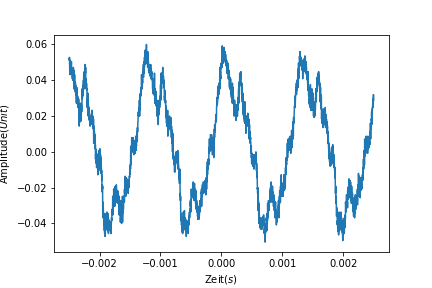
\includegraphics[width=11cm]{messwerteharmonika.png}
	\caption{Das aufgenommene Signal der Mundharmonika}
\end{figure}
\section{Auswertung}
\label{chap:VERSUCH_1_AUSWERTUNG}

\begin{table}[H]
\centering
\begin{tabular}{|l|l|l|}
\hline
\multicolumn{1}{|c|}{} & \multicolumn{1}{c|}{Ergebnis}						\\ \hline
Grundperiode in ms						&$1.244$							\\ \hline
Grundfrequenz in Hz						&$803.8585$							\\ \hline
Signaldauer in s						&$0.005$							\\ \hline
Abtastfrequenz in Hz					&$500000$							\\ \hline
Signallänge M							&$2500$								\\ \hline
Abtastintervall in s					&$0.000002$							\\ \hline
\end{tabular}
\caption{}
\end{table}

Die Frequenzachse des numerisch berechneten Spektrums ist in der Einheit Anzahl Schwingungen innerhalb der gesamten Signaldauer,d.h.der n-teEintragimSpektrum f[n] entspricht n Schwingungen innerhalb der Gesamtlänge des Signals von M $\Delta{t} s$. Die zugehörige Frequenz f in Hertz berechnet sich folglich aus $$f=\frac{n}{M{\cdot}\Delta{t}}$$
 
\begin{figure}[H]
	\centering\small
	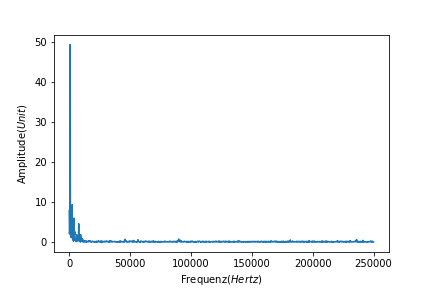
\includegraphics[width=11cm]{Spektrum.png}
	\caption{Das Spektrum von dem aufgenommenen Signal der Mundharmonika}
\end{figure}

Den Code davon bitte den Anhang A.1.1 sehen.

\section{Interpretation}
\label{chap:VERSUCH_1_INTERPRETATION}
Die Note G sollte normalerweise ungefähr die Frequenz 770 Hz haben. Wir haben aber 803 Hz(ca. Note G\#) berechnet. Das könnte sein, dass wir nicht ganz genau G gespielt haben, weil beim Spielen einer Mundharmonika auch in gleiche Öffnung mit unterschiedlicher Weise(blasen oder ziehen, mit gedrücktem Schieber oder nicht) man unterschiedliche Noten bekommen würde.

Aus dem Spektrum kann man die Grundfrequenz ablesen, da bei der der Höchstpunkt von dem Graph liegt. Diese Grundfrequenz beträgt 800 Hz. Und die Amplitude von dieser Fourierkomponente ergibt sich $49.466575158710356$.

%
% CHAPTER Versuch 2
%
\chapter{Frequenzgang von Lautsprechern}
\section{Fragestellung, Messprinzip, Aufbau, Messmittel}
\qquad Mikrofon mit Oszilloskop bei Kanal 1, Lautsprecher(groß und klein) bei Kanal 2 verbinden.
Generator(Quelle von den Lautsprechern) generiert Storm in Form von Sinusschwingung verschiedener Frequenz.

Die Frequenz kann bei Generator eingestellt werden(100,200,300,400,500,700,850 Hz, 1, 1.2, 1.5, 1.7, 2 kHz, 3, 4, 5, 6, 10 kHz). Für jede Frequenz, die man misst, muss die Spannung auf 1,5 V eingestellt werden, damit die Amplitude von Eingangsignal nicht ändert.

Eingangssignal(von den Lautsprechern) und Ausgangssignal(von dem Mikrofon) sind zu protokollieren. Beide Lautsprechern müssen den gleichen Abstand zum Mikrofon haben und das beide Kanäle auf AC \textit{coupling} gestellt sind.

Die Amplituden- und Phasengang sind grafisch darzustellen. Daher wird mithilfe von matplotlib(mit der Funktion semilogx()) ein Bode-Diagramm erstellt werden. Die zugehörigen Angaben werden entsprechend in Dezibel und Phasenwinkel umgewandelt.

\section{Messwerte}
\label{chap:VERSUCH_2_MESSWERTE}
\begin{figure}[H]
	\centering\small
	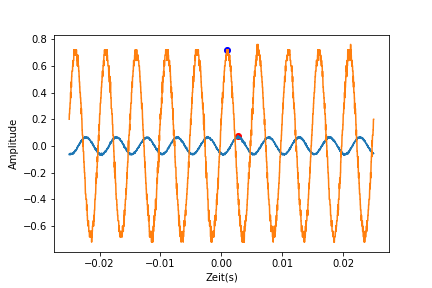
\includegraphics[width=11cm]{gross200Hz.png}
	\caption{Beispiel: Ein-Ausgangssignal mit Höchstpunkten bei Frequenz 200Hz von dem großen Lautsprecher}
\end{figure}
\begin{figure}[H]
	\centering\small
	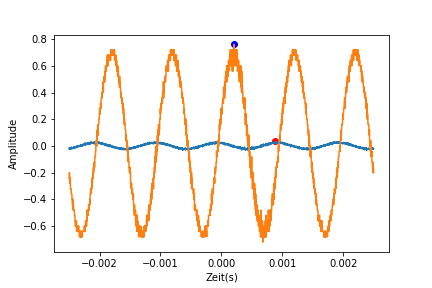
\includegraphics[width=11cm]{gross1000Hzk.png}
	\caption{Beispiel: Ein-Ausgangssignal mit Höchstpunkten bei Frequenz 1kHz von dem kleinen Lautsprecher}
\end{figure}
\section{Auswertung}

\label{chap:VERSUCH_2_AUSWERTUNG}

Da die beide Signal nicht gleichzeitig kommen, entsteht eine Phasenverschiebung. Die haben wir hergeleitet, indem wir die Höchstpunkt vom Ausgangssignal finden und mit dem direkt vorher liegenden Höchstpunkt vom Eingangssignal vergleichen. Die Differenz von beiden Höchstpunkten sind die Phasenverschiebung in Sekunde. Die Amplitudengang  gibt für jede Frequenz an, wie die einzelnen Sinusschwingungen verstärkt oder abgeschwächt werden. Die Amplituden werden grob mit Höchstpunkt bestimmt.


\begin{table}[H]
\centering
\begin{tabular}{|l|l|l|}
\hline
\multicolumn{1}{|c|}{Frequenz} & \multicolumn{1}{c|}{Amplitudengang}		& \multicolumn{1}{c|}{Phasenverschiebung}			\\ \hline
100 Hz						&$0.03567568$			&$0.00962$				\\ \hline
200 Hz						&$0.10105263$			&$0.00186$				\\ \hline
300 Hz						&$0.06842105$			&$0.00174$				\\ \hline
400 Hz						&$0.05263158$			&$0.0016$				\\ \hline
500 Hz						&$0.04315789$			&$0.00118$				\\ \hline
700 Hz						&$0.031$				&$0.00104$				\\ \hline
850 Hz						&$0.03263158$			&$0.0008$				\\ \hline
1000 Hz						&$0.04631579$			&$0.000564$				\\ \hline
1200 Hz						&$0.03684211$			&$0.00052$				\\ \hline
1500 Hz						&$0.03368421$			&$0.000496$				\\ \hline
1700 Hz						&$0.03684211$			&$0.000502$				\\ \hline
2000 Hz						&$0.03333333$			&$0.000402$				\\ \hline
3000 Hz						&$0.033$				&$0.00031$				\\ \hline
4000 Hz						&$0.03692308$			&$0.000033$				\\ \hline
5000 Hz						&$0.029$				&$0.0000584$				\\ \hline
6000 Hz						&$0.02888889$			&$0.0000728$				\\ \hline
10000 Hz					&$0.02842105$			&$0.0000988$				\\ \hline
\end{tabular}
\caption{Großer Lautsprecher}
\end{table}


\begin{table}[H]
\centering
\begin{tabular}{|l|l|l|}
\hline
\multicolumn{1}{|c|}{Frequenz} & \multicolumn{1}{c|}{Amplitudengang}		& \multicolumn{1}{c|}{Phasenverschiebung}			\\ \hline
100 Hz						&$0.02105263$			&$0.00907$				\\ \hline
200 Hz						&$0.02947368$			&$0.00072$				\\ \hline
300 Hz						&$0.03$					&$0.00063$				\\ \hline
400 Hz						&$0.04421053$			&$0.000762$				\\ \hline
500 Hz						&$0.08315789$			&$0.00066$				\\ \hline
700 Hz						&$0.06$					&$0.000986$				\\ \hline
850 Hz						&$0.05263158$			&$0.000764$				\\ \hline
1000 Hz						&$0.04421053$			&$0.000684$				\\ \hline
1200 Hz						&$0.03263158$			&$0.000634$				\\ \hline
1500 Hz						&$0.03263158$			&$0.00064$				\\ \hline
1700 Hz						&$0.03157895$			&$0.000486$				\\ \hline
2000 Hz						&$0.03263158$			&$0.000426$				\\ \hline
3000 Hz						&$0.03578947$			&$0.000318$				\\ \hline
4000 Hz						&$0.02631579$			&$0.000018$				\\ \hline
5000 Hz						&$0.034$				&$0.000056$				\\ \hline
6000 Hz						&$0.02210526$			&$0.000028$				\\ \hline
10000 Hz					&$0.027$				&$0.000013$				\\ \hline
\end{tabular}
\caption{Kleiner Lautsprecher}
\end{table}



\textit{Zeit in Phasenwinkel umwandeln:} $$\varphi{_H}=-{\Delta}t{\cdot}f{\cdot}360^{\circ}$$
\textit{Amplitudengang in Dezibel umwandeln:}$$20{\cdot}\log_{10} (Amplitudengang)$$


\begin{figure}[H]
\centering\small
\fbox{
	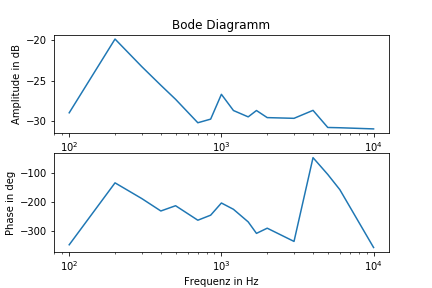
\includegraphics[width=11cm]{bodediagrammgr.png}
	}
	\caption{Bode-Diagramm von dem großen Lautsprecher}
\end{figure}

\begin{figure}[H]
\centering\small
\fbox{
	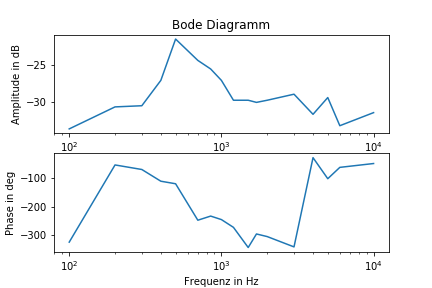
\includegraphics[width=11cm]{bodediagrammkl.png}
	}
	\caption{Bode-Diagramm von dem kleinen Lautsprecher}
\end{figure}

Den Code davon bitte den Anhang A.1.2 sehen.

\section{Interpretation}
\label{chap:VERSUCH_2_INTERPRETATION}
Bei der Tabelle von dem Amplitudengang kann man einsehen, dass die Veränderung von Amplituden am Anfang groß ist aber danach tendenziell absteigt, da bei zu klein Frequenz die Geräusch nicht laut genug ist. Bei wachsenden Frequenzen braucht immer mehr Energie, dass die Geräusche leiser werden.
Bei zu kleinen Frequenzen(100-200Hz) und zu großen Frequenzen (5000-10000Hz)sind die Phasengang im Bode-Diagramm sind nicht wie erwartet(aufsteigend, absteigend dann wieder aufsteigend, große überraschende Sprünge). Der Grund dafür könnte sein, dass die Lautsprecher bei zu groß oder zu klein Frequenzen nicht richtig annehmen können.


%
% CHAPTER Anhang
%
\renewcommand\thesection{A.\arabic{section}}
\renewcommand\thesubsection{\thesection.\arabic{subsection}}

\chapter*{Anhang}
\label{chap:APPENDIX}
\addcontentsline{toc}{chapter}{Anhang}
%\setcounter{chapter}{0}
\addtocounter{chapter}{1}
\setcounter{section}{0}

\section{Quellcode}
\label{chap:APPENDIX_SOURCECODE}

\subsection{Quellcode Versuch 1}
\label{chap:APPENDIX_SOURCECODE_V1}
\begin{lstlisting}[
style=PYTHON,
frame=single,
caption=,
captionpos=b,
label=lst:V1]
#from TekTDS2000 import *
import numpy as np
import matplotlib.pyplot as plt
#scope = TekTDS2000()

data = np.genfromtxt("harleybentonrichtig.csv", delimiter=",")
datas = data[:,1]
dataz = data[:,0]

ind = np.argmax(datas)
print(ind)
ind2 = np.argmax(datas[ind + 1:]) + ind + 1
print(ind2)
periode = dataz[ind2]-dataz[ind]
print("grper", periode)
gfre = 1/periode
print("grfre", gfre)

sigdauer = 0.005 #5ms
ablen = len(data) #Signallänge
abin = sigdauer / ablen #abtastinterval
abfr = 1 / abin #abtastfrequenz
print("Signaldauer: ", sigdauer)
print("Abtastfrequenz: ", abfr)
print("Signallänge: ", ablen)
print("Abtastintervall: ", abin)


Y = abs(np.fft.fft(datas)) # fft computing and normalization
schw = np.argmax(Y)
Y = Y[range(1250)]
plt.xlabel('Frequenz($Hertz$)')
plt.ylabel('Amplitude($Unit$)')
x = np.linspace(0,abfr/2,1250,endpoint = True)
plt.plot(x,abs(Y))
plt.savefig("Spektrum.png")
plt.show()

plt.xlabel('Zeit($s$)')
plt.ylabel('Amplitude($Unit$)')
plt.plot(dataz,datas)

print('Grundfrequenz: ', schw/(ablen * abin))
print('Amplitude: ', np.max(Y))
\end{lstlisting}

\subsection{Quellcode Versuch 2}
\label{chap:APPENDIX_SOURCECODE_V2}
\begin{lstlisting}[
style=PYTHON,
frame=single,
caption=,
captionpos=b,
label=lst:V2]
import numpy as np
import matplotlib.pyplot as plt

def verschieb(hz):
    per = int((1/hz)/zeitUnit)

    ind1 = np.argmax(data1)
    if (ind1 - per) < 0:
       ind1 = ind1 + per
    ind2 = ind1 - per + np.argmax(data2[ind1-per:ind1])
    
    verschiebung = dataz[ind1] - dataz[ind2]
    plt.plot(dataz[ind1],data1[ind1],"ro")
    plt.plot(dataz[ind2],data2[ind2],"bo")
    print('Verschiebung: ' + str(verschiebung) + 's')
    return(verschiebung)

amp = np.zeros(17)
phase = np.zeros(17)

index = [100,200,300,400,500,700,850,1000,1200,1500,1700,
      2000,3000,4000,5000,6000,10000]
c = 0
for i in index:
    data = np.genfromtxt(str(i) + "Hzk.csv", delimiter=",")
    data1 = data[:,1]
    data2 = data[:,2]
    dataz = data[:,0]
    zeitUnit = dataz[1]-dataz[0]
    phase[c] = round(verschieb(i),10)
    amp[c] = np.max(data1)/np.max(data2)

    c = c + 1
    plt.ylabel('Amplitude')
    plt.xlabel('Zeit(s)')
    plt.plot(dataz,data1)
    plt.plot(dataz,data2)
    if (i == 1000):
        plt.savefig("gross1000Hzk.png")
    plt.show()
    
print('-------Amplitude--------')   
print(amp)
plt.title('Amptitudengang')
plt.plot(index,amp)
plt.show()
print('-------Verschiebung--------')
print(phase)
plt.title('Phasengang')
plt.plot(index,phase)
plt.show()

db = 20*np.log10(amp)
Phasenwinkel = -phase*index*360
print('---------------')
print(db)
print('---------------')
print(Phasenwinkel)
plt.subplot(2,1,1)
plt.title('Bode Diagramm')
plt.semilogx(index,db)
plt.ylabel('Amplitude in dB')
plt.subplot(2,1,2)
plt.semilogx(index,Phasenwinkel)
plt.ylabel('Phase in deg')
plt.xlabel('Frequenz in Hz')
plt.savefig("bodediagrammkl.png")
\end{lstlisting}

\end{document}
%------------------------------------
% ╔═╗╔╗╔╔╦╗  ╔╦╗╔═╗╔═╗╦  ╦╔╦╗╔═╗╔╗╔╔╦╗
% ║╣  ║║║  ║║     ║║║  ║║    ║  ║║║║║ ╣  ║║║ ║ 
% ╚═╝╝╚╝═╩╝  ═╩╝╚═╝╚═╝╚═╝╩  ╩╚═╝╝╚╝  ╩ 
%------------------------------------